\subsection{Server}
Server funguje na základe jedného jednoduchého skriptu, ktorý je napísaný v jazyku Python, konkrétne hovoríme o frameworku Flask.

Logika Flasku je celkom priamočiara. Pre rôzne url endpointy vykoná inú funkciu. Základom je anotácia \texttt{@app.route('/pripona/url')} \cite{flask_approute}, kde jedným z parametrov do funkcie \texttt{route()} je reťazec, ktorý symbolizuje url endpoint, pre ktorý sa má funkcia vykonať. Definícia funkcie a jej telo nasledujú hneď za \texttt{@app.route()}. 

Pre ukážku povedzme, že server funguje na doméne \texttt{https://flask.website.com}. Potom, ak existuje nasledujúci kód:
\newline
\begin{lstlisting}[language=Python, basicstyle=\small]
@app.route('/test')
def function():
    currentDate = datetime.now().strftime('%d/%m/%Y %H:%M:%S')
    return 'Hello World! ' + currentDate
\end{lstlisting}
\leavevmode\newline
Tak po zadaní url \texttt{https://flask.website.com/test} sa zobrazí text

\begin{center}
    \textit{Hello World! 26/5/2020 22:55:32}
\end{center}
(čas, keby sme zadali url v čase písania tohto textu).

Všetky dáta, ktoré server uchováva sú dočasné. Preto je rozumné použiť pamäť RAM. Ešte lepšie je použiť cache, ktorá je súčasťou RAM a ponúka ešte rýchlejší prístup k dátam. Takzvaný ,,memory caching'' je technika, kedy aplikácie dočasne ukladajú svoj obsah do časti pamäte RAM, ktorá sa volá cache \cite{cache}.

\begin{figure}[ht]
  \centering
  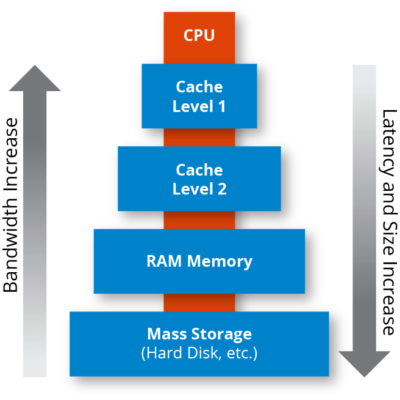
\includegraphics[width=8cm]{img/cache.png}
  \caption{Porovnanie rôznych typov pamäte v závislosti od rýchlosti a kapacity.}
  \label{cache}
\end{figure}

Keď sa aplikácia pokúša čítať dáta, najprv skontroluje, či nie sú v cache. Ak nie, prečíta ich z databázy, čo trvá dlhšie. Následne ich zapíše do cache, aby najbližšie čítanie daného záznamu bolo rýchlejšie. Tým, že cache má limitovaný ukladací priestor, je dôležité vymyslieť stratégiu, ako staré dáta mazať a nahrádzať novými. 

Cache je vysoko favorizovaná najmä ak ide o časté a opakované úkony. Ak pristupujeme k určitým dátam na pravidelnej báze, je lepšie uchovávať ich v cache, aby nemusela byť prehľadávaná celá databáza, respektíve súbory vo filesystéme.

Opísali sme ako sa cache používa v najčastejších prípadoch. My sme sa rozhodli pozerať na cache trochu inak. Náš server nemá žiadnu databázu. Ani sa na žiadnu nenapája. Jediné, čo má, je cache. Každý záznam v nej je jedinečný a po jeho použití zmizne. Takže rovnako tu nejde o opakované úkony k rovnakým dátam. 

Zopakujeme ešte raz fakt, že všetky dáta servera sú dočasné. Preto považujeme za kontraproduktívne a neefektívne vytvoriť databázu a pristupovať k nej pri výbere dát. Cache je rýchla, jej veľkosť je postačujúca. Komplexita je minimálna. Toto je dôležitý faktor, nakoľko komplexita je najväčší nepriateľ bezpečnosti. V Pythone je jej implementácia jednoduchá. Dáta nemusíme šifrovať. Tým nám odpadá problém bezpečného ukladania šifrovacích kľúčov.

Na implementáciu cache v Pythone budeme používať Werkzeug knižnicu \cite{werkzeug_cache}. Na začiatku si vytvoríme jej inštanciu \texttt{cache = SimpleCache()}. Následne ju môžeme používať. V kóde neskôr používame jej tri najčastejšie metódy a to: \texttt{cache.set()} (pri pridávaní nových dát), \texttt{cache.get()} (pri verifikácii) a \texttt{cache.delete()} (po úspešnej verifikácii).
